\subsection{Taxi Status Duration}
The duration distribution for each status are shown in Fig.~\ref{figure_duration_for_each_status}. Status duration represents the time length of a taxi staying in a certain status. The red line presents the duration time distribution for vacant status, and the green one is for occupied status. Note that the red line (vacant status) approaches to  one earlier than than the blue line (occupied status). So the value of vacant duration is smaller than the value of occupied duration. This is reasonable since drivers tend to shorten the waiting time to raise their incomes.
\begin{figure}[!h]
\centering
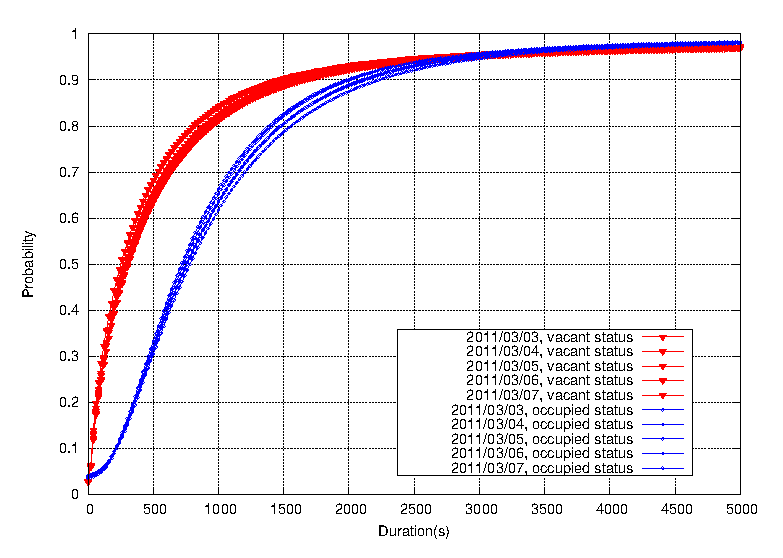
\includegraphics[width=0.38\textwidth]{figures_201103/assumption/durationdis.eps}\\
\caption{Status duration distributions.}\label{figure_duration_for_each_status}
\end{figure}

Overall, the statistical results for both speed and status duration are consistent with \emph{Claim 1}, that is, the behaviors of taxis are similar within each status while differ between the two statuses.
